\chapter{Développement}
\section{Technologies utilisées}
\subsection{NodeJs}
Aux alentours de 2010 Google a commencé à rendre JavaScript et son moteur d'exécution V8 plus rapides. Des outils comme Node.js sont ensuite apparus\cite{NodeJs}.\newline
Node.js est un environnement d'exécution \textbf{JavaScript} construit sur le moteur \emph{V8} de Google Chrome. Il utilise un modèle basé sur l'événementiel (\textbf{event-driven}) et des entrées/sorties non bloquantes, ce qui le rend léger et efficace.
Il présente plusieurs avantages, notamment :
\begin{itemize}
	\item NodeJS et son écosystème permettent de travailler avec JavaScript à la fois sur le frontend et le backend.
	\item L'approche non bloquante de NodeJs lui permet d'effectuer des entrées/sorties (I/O) de manière asynchrone. La programmation asynchrone est idéal pour une exécution plus rapide de programmes.
	\item Contrairement aux langages serveur célèbres tel que PHP, ASP.NET, Ruby ou Java. Node Js s'exécute en \emph{monothread}, en d'autres termes les processus de chaque requêtes sont traités dans un seul fil d'exécution, ce qui est très efficace en termes de mémoire.
	\item NodeJs rassemble une grande communauté très active, ce qui offre un grand nombre de librairies et de support en travaillant avec NodeJs.\newline
\end{itemize}
NodeJs est donc un choix idéal pour des développer des APIs REST minimales et flexibles tout en gardant des performances élevées pendant le traitement de requêtes.\newline
En dernier, bien que NodeJs ne soit pas adapté pour des applications aux calculs intensives, il ne sera pas un inconvénient du fait que les calculs sur le graphe seront effectués principalement dans le SGBD.

\subsection{MongoDB}
	MongoDb est un système de base de données NoSQL. Il est orienté documents qui est une évolution des simples bases de données clé-valeur, un document peut être une valeur atomique, paire clé-valeur, un tableau de valeurs ou une compositions de ces derniers.

Son nom vient de Humongous qui veut dire énorme ou immense.

\subsection{Neo4J}
Apparu en l'année 2000 et appartient à la société Neo Technology, Neo4j est un système de gestion de bases de données (SGBD) orienté graphe. Son approche est fondée sur la théorie des graphes. Les données sont stockées de manière assez libre (sans modèle prédéfini) dans des nœuds reliés entre eux par des relations.

Ses principaux avantages sont :
\begin{itemize}
	\item Neo4J utilise un stockage native du graphe, avec un principe appelé \textbf{index-free adjacency}, ceci permet de stocker des nœuds directement avec ses relations et nœuds adjacents sans avoir à utiliser des indexes pour consulter ses relations.\newline
	Le stockage native offre de très grande performances de lecture/écriture indépendamment de la taille du graphe (le temps d'accès à chaque noeud est constant).
	\item Neo4J est open-source, et a la plus grande communauté dans les bases de donnée orientées graphe, qui contribuent constamment à son écosystème, ce qui donne un très grand nombre de ressources et de support ainsi qu'une grande liste de pilotes et librairies dans tous les langages courants.
	\item Neo4J se présente comme une solution dans un très grand nombre de cas d'utilisations, par exemple: Réseaux sociaux, détection de fraude, Réseaux et opérations IT...etc.
	\item Facile à apprendre et à utiliser: Neo4J dispose d'une interface graphique très moderne et riche, et utilise son propre langage d'interrogation Cypher qui utilise une syntaxe textuelle très intuitive et similaire au SQL.
\end{itemize}

Neo4J étant le SGBD le plus dominant dans le domaine des orientés graphe, et offrant une grande performance et flexibilité qui satisfait tous les besoins de ce projet, nous n'avons pas eu besoin de considérer les autres systèmes.

\textbf{Cypher: } c'est un langage de requête déclaratif sur Neo4J. Il permet de décrire la forme du résultat et les contraintes souhaitées à ajouter en optimisant le plan d'exécution pour récupérer les résultats.\newline

Il utilise une syntaxe déclarative avec de l'ASCII Art pour décrire les nœuds et les relations, rendant les requêtes faciles à lire et comprendre. un exemple est donné dans la figue \ref{fig:cypher}.

\begin{figure}
	\center
	\includegraphics[width=0.8\textwidth]{img/cypher.png}
	\label{fig:cypher}
	\caption{Exemple de requête Cypher.}
\end{figure}
		
\section{Structure de l'application}
\subsection{L'architecture MVC (Model-View-Controller)}
L'application suit une architecture MVC qui est un modèle d'architecture qui sépare une application en 3 composants logiques: \textbf{Model}, \textbf{View}, \textbf{Controller}.
Chaque composant est construit pour gérer un aspect spécifique de l'application, on peut résumer le rôle de chacun comme suit :
\begin{enumerate}
	\item \textbf{Models: } ces composants correspondent à tout ce qui est relié aux données, un model peut représenter une classe d'objets ou une structure de données échangée entre Views et Controllers, ainsi que la logique manipulant ces données tel que des calculs de moyennes ou les différentes opérations d'ajout, modification et suppression dans une base de données.
	\item \textbf{Views:} les views sont utilisés pour l'interface utilisateur (UI) de l'application, ceci inclut les composants d'interface (Textes, boutons, formulaires...etc.), ainsi que certaines logiques de mise en forme et affichage des données.
	\item \textbf{Controller: } le Controller joue le rôle d'une interface entre le Model et les Views afin de traiter les requêtes venant du View (Par exemple un clique de bouton), manipuler les données du Model et enfin les rendre au View pour qu'elles soient présentées. il contient généralement la logique des actions effectuées par l'utilisateur.
\end{enumerate}
	
MVC est une des architectures les plus utilisées pour créer des projets évolutifs et extensibles \cite{refMVC}.
%Il existe plusieurs variantes du MVC et d'autres architectures similaires tel que le MVVM (Model-View-ViewModel) et le MVP (Model-View-Presenter).

\subsection{Composants de l'application}

\begin{figure}
	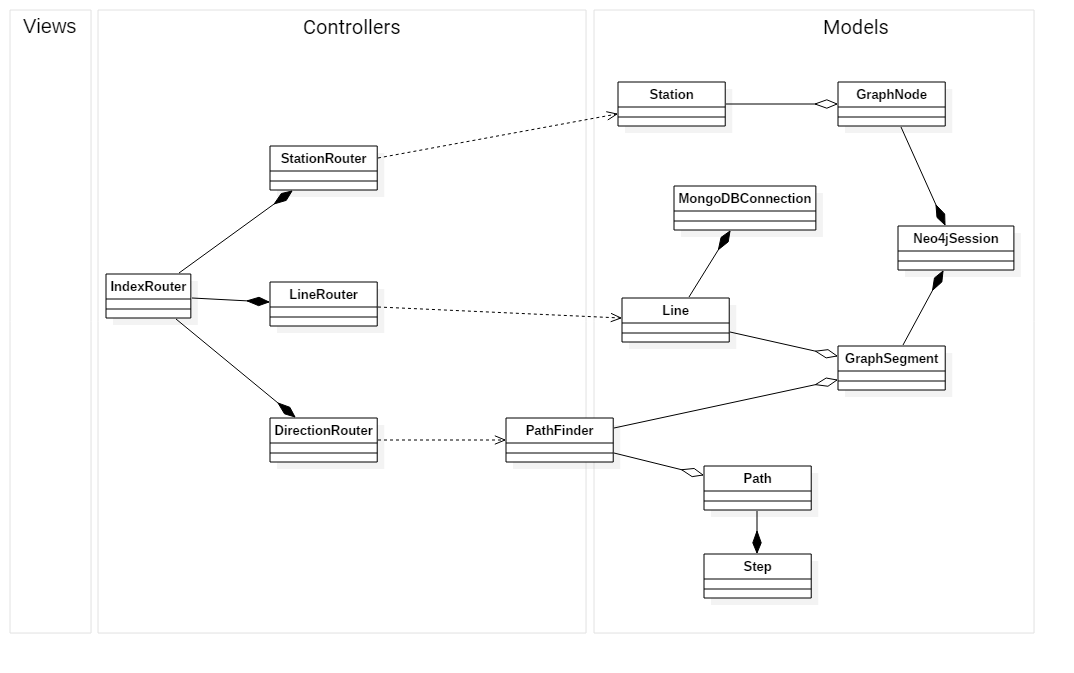
\includegraphics[width=\textwidth]{img/ClassDiagram.png}
	\caption{Vue d'ensemble des composants de l'application}
	\label{fig:classDiagram}
\end{figure}	
\begin{enumerate}
	\item \textbf{Models:}
	      \begin{itemize}
	      	\item \textbf{Station} : représente une station avec son nom, adresse et coordonnées.
	      	\item \textbf{Line} : représente une ligne de transport, le format complet est décrit dans la partie \ref{ref:resources}.
	      	      \begin{itemize}
	      	      	\item \textbf{Bus} : représente un Bus ainsi que les différents facteurs estimés (temps d'attente moyen, fréquence ...etc.).
	      	      \end{itemize}
	      	\item \textbf{Path} : représente une suggestion de chemin, contient les informations globales tel que le prix et temps total du chemin, ainsi qu'une liste d'objets Step.
	      	      \begin{itemize}
	      	      	\item \textbf{Step} : représente une étape d'un itinéraire utilisant le même moyen de transport, comporte la station de départ et d'arrivée, les stations intermédiaires et les informations sur le temps, cout et distance à parcourir.
	      	      \end{itemize}
	      	      le format de cet objet est détaillé dans la section \ref{ref:formatReponse}
	      	\item \textbf{Models du graphe} : 
	      	      Afin d'avoir une application facilement extensible, nous avons séparé les Models relatifs au graphe des Models de l'application, ce qui permettra de modifier la représentation du graphe sans affecter l'application.
	      	      \begin{itemize}
	      	      	\item \textbf{GrapheNode} : représente un nœud, communique avec la base de donnée pour créer et manipuler les nœuds.
	      	      	\item \textbf{GrapheSegment} : représente un arc entre deux nœuds, communique avec la base de donnée pour créer plusieurs relations (lignes de transport) ou les supprimer.
	      	      \end{itemize}
	      \end{itemize}
	      	
	\item \textbf{Controller :} dans le cas de notre application, le controller est le \emph{router} de l'application, ce dernier permet de définir les différents points terminaux (endpoints) de l'application et les identifier par une URI, les détails de l'API sont décrits dans la section suivante.
	      
	      Nous avons utilisé dans l'implémentation \textbf{ExpressJs} : un framework\FancyFootNote{Framework : C'est une sorte d'infrastructure de développement, il désigne un ensemble cohérent de composants logiciels structurels qui sert à créer les fondations ainsi que les grandes lignes de tout ou d'une partie d'un logiciel ou application.} d'application minimaliste et très flexible qui propose un ensemble de fonctionnalités stables pour les applications web, en l'occurrence l'implémentation des APIs (Express.Router). Au moment d'écrire ce rapport, c'est l'outil le plus connu et le plus utilisé avec NodeJs.
	      	
	\item \textbf{Views :} les Views dans ce projet consistent en deux applications séparées : une application client pour demander le chemin et consulter les lignes, et une application admin pour insérer et modifier les lignes des différents transports.
	      
	      Ces deux applications sont des \emph{Single Page Applications} : une application dynamique qui tourne sur un navigateur web.
	      Nous ne détaillerons pas l'implémentation de ces applications car ce n'est pas l'objectif principal de ce projet, un aperçu du résultat final est donné dans la section \ref{ref:Implementation}.
\end{enumerate}
	
	
	
\section{Implémentation de l'API}
\label{ref:API}
\subsection{Ressources exposées}
Notre API définit principalement 3 ressources:
\begin{enumerate}
	\item \textbf{Station:} Ressource qui représente les différentes stations du réseau, elle accepte 3 requêtes différentes de type GET  : 
	      \begin{itemize}
	      	\item \emph{\textbf{/api/station}}: Retourner toutes les stations, peut être utilisée pour visualiser toutes les stations par un client ou d'autres utilisations générales, le nombre de stations retournées seront limités et contrôlés par deux paramètres \textbf{limit} et \textbf{offset} afin d'éviter de retourner un très grand nombre de stations en une seule requête.
	      	\item \emph{\textbf{/api/station/\{id\}}}: Retourner une station par identifiant, le client n'ayant rarement besoin de l'identifiant, cette URI est généralement utilisée dans le coté administrateur.
	      	\item \emph{\textbf{/api/station?match=\{name\}}}: Un paramètre dans la ressource station permet de retourner toutes les stations dont le nom contient la valeur \emph{name}, peut être utilisé pour la recherche et auto-complétion lors du choix du chemin, par exemple.
	      \end{itemize}
	      	      			
	      Cette ressource accepte aussi des requêtes de type POST (création), PUT (mise à jour) et DELETE (suppression)  pour les client admin (authentifiés).
	\item \textbf{Ligne:} \emph{\textbf{/api/line}} : Ressource qui représente les différentes lignes de transport entre stations, elle accepte des requêtes de type GET du coté client, aussi des requêtes POST, PUT et DELETE du coté admin pour gérer les lignes.
	\item \textbf{Direction:}  \emph{\textbf{/api/direction}} : Ressource représentant les chemins, elle accepte seulement des requêtes de type GET, les détails de ces requêtes et leurs réponses sont détaillés dans la section \ref{SectionPathFinding}
\end{enumerate}
\subsection{Description des formats des ressources}
Les ressources principales de notre API sont les stations (\textbf{station}) et les lignes (\textbf{line}), leur format est décrit dans la figure \ref{fig:formatResources}.
\label{ref:resources}
% Format JSON 
\lstset{style=JSON}

\begin{figure}[h!]
	%-------------------------------------------------------------------
	\begin{subfigure}[b]{0.45\linewidth}
		\begin{lstlisting}[caption=Format JSON de Station]
{
	ID: 1,
	name: "string",
	address: "string",
	coords: 
	[
	  {
	  	  direction: "string",
  		  lat: 0.00,
   		  lon: 0.00
	  }
	]
}
		\end{lstlisting}
	\end{subfigure}\hfill%  
	%-------------------------------------------------------------------
	\begin{subfigure}[b]{0.45\linewidth}
		\begin{lstlisting}[caption=Format JSON de Line]
{
  "id": 0,
  "name": "string",
  "bus": {
    "name": "string",
    "price": 0,
    "frequence": 0,
    "avgWaitTime": 0
  },
  "lineStations": [
    {
      "stationID": 0,
      "distFromPrev": 0,
      "timeFromPrev": 0
    }
  ]
}
		\end{lstlisting}
	\end{subfigure}\hfill%  
	%-------------------------------------------------------------------
	\caption{Description du format des ressources.}
	\label{fig:formatResources}
\end{figure}

\section{Recherche de chemin}
L'implémentation de l'application du coté serveur permet de calculer un ensemble de chemins optimaux entre deux stations identifiées par un identifiant. Le calcul se déroule en plusieurs étapes :
\subsection{Déroulement d'une requête}

\begin{figure}[h!]
	\center
	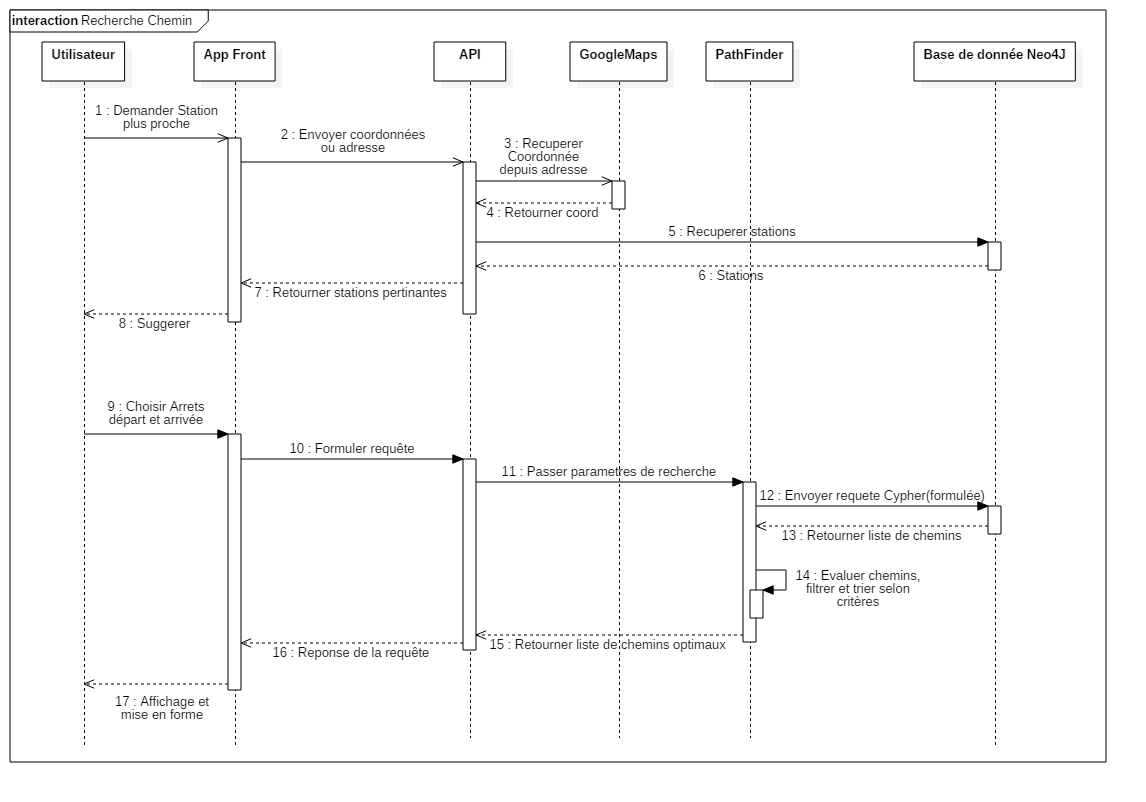
\includegraphics[width=0.99\textwidth]{img/RechercheChemin.png}
	\caption{Diagramme de séquence pour la recherche de chemins.}
	\label{fig:diagSequence}
\end{figure}

Une requête de chemin à partir de l'utilisateur jusqu'à l'affichage de la réponse passe par plusieurs étapes, la figure \ref{fig:diagSequence} décrit les étapes suivantes :


\begin{enumerate}
	\item L'API reçoit la requête de chemin, vérifie les paramètres et met en forme les données, pour les passer au module qui calcule le chemin (PathFinder).
	\item Le module PathFinder formule la requête Cypher et l'envoi au serveur de la base de donnée Neo4j.
	      Un exemple de cette requête est donné dans la figure \ref{fig:cipherRequest}.
\begin{figure}[h!]
	      \begin{lstlisting}[style=cypher]
MATCH p = AllShortestPaths((A:Station)-[*..20]->(B:Station))
WHERE A.name = {startParam} AND B.name = {endParam}
	AND ALL(rel IN relationships(p) 
	WHERE type(rel) IN {transportsParam})

WITH p, RELATIONSHIPS(p) as segments
WITH EXTRACT (segment in segments| StartNode(segment)) AS startNodes,
EXTRACT (segment in segments| EndNode(segment)) AS endNodes,
RELATIONSHIPS(p) as segments
            
RETURN segments, startNodes, endNodes
	      \end{lstlisting}
\caption{Requête Cypher des plus courts chemins}
\label{fig:cipherRequest}
\end{figure}
	      Nous pouvons depuis cette requête filtrer les différents transports à inclure dans le chemin facilement, puisque chaque moyen de transport est désigné par ses propres arcs étiquetés dans le graphe.
	\item Neo4J retourne ainsi une liste de chemins optimaux, le module va ensuite évaluer chaque chemin :
	      \begin{itemize}
	      	\item Évaluer le temps et cout estimé de chaque chemin.
	      	\item Trier les chemins selon le critère de la requête, en cas d'égalité considérer les autres critères.
	      	\item Structurer chaque chemin en Objets Path, détaillé dans la section suivante.
	      	\item Minimiser le chemin en regroupant les étapes intermédiaires (tel que deux arrêts utilisant le même Bus).
	      \end{itemize}
	\item Retourner l'objet à l'API qui l'envoi sous forme de réponse HTTP.
\end{enumerate}
\label{SectionPathFinding}
	
%\subsection{Format des requêtes}
%**Montrer une requete HTTP du chemin avec les parametres ? 
\subsection{Format des réponses}
\label{ref:formatReponse}
L'API retourne un tableau des chemins (tableau d'objets Path) en format JSON, ces objets contiennent les informations suivantes :
\begin{itemize}
	\item Le temps, prix et distance totale du chemin.
	\item Les moyens de transport utilisés dans ce chemin.
	\item La liste des étapes à suivre dans ce chemin, chaque étape contenant les données suivantes:
	      \begin{itemize}
	      	\item La station de départ et la station d'arrivée.
	      	\item Les stations intermédiaires entre station de départ et d'arrivée.
	      	\item Le prix, temps estimé et distance à parcourir de l'étape.
	      	\item Le transport à prendre (ou type de l'étape).
	      \end{itemize}
\end{itemize}

\begin{figure}
\begin{lstlisting}[]
{
  "totalDist": 0,
  "totalPrice": 0,
  "totalTime": 0,
  "steps": [
    {
      "sourceStation": {
        "id": 0,
        "name": "string",
        "address": "string",
        "coordLat": 0,
        "coordLon": 0
      },
      "destStation": {
        "id": 0,
        "name": "string",
        "address": "string",
        "coordLat": 0,
        "coordLon": 0
      },
      "price": 0,
      "time": 0,
      "type": "string",
      "name": "string"
    }
  ]
}
\end{lstlisting}
\caption{Format JSON de Path (chemin)}
\end{figure}

\section{Implémentation}
\label{ref:Implementation}